% Latex / Beamer template for the Georgia Tech's CS6476 class.
% This template is set to render images that are located in the output 
% folder. The following directory structure has been assumed:
%
% psXY/
%     output/
%         psX-a-b-c.png
%         psX-d-e-f.png
%         ...
%     this_file.tex
%
% If a different structure is used, the images path must be changed in 
% each call of \begin{figure} ... \end{figure}
%
% Your Name and email address must be added in the \author definition.
%
% This file is set initially as a draft as showed in the \documentclass statement. 
% In order for the your images to show, the 'draft' option should be removed or 
% replaced by 'final'. Please note that once this feature is changed, there will be 
% compilation errors if an image cannot be found.

\documentclass[aspectratio=169]{beamer}

\usepackage{tikz}
\usepackage[font={bf, small},labelformat=empty]{caption}
\usepackage[caption=false]{subfig}
\captionsetup[subfigure]{labelformat=empty, font={bf, Large}}

\setbeamertemplate{itemize items}[ball]
\setbeamercolor*{item}{fg=black}
\usefonttheme{structurebold}

\usebackgroundtemplate{
	
\begin{tikzpicture}
	\shade [outer color = gray!20, inner color = white]
	(0,0) rectangle (\paperwidth,\paperheight);
	\end{tikzpicture}}

\setbeamerfont{title}{series=\bfseries,parent=structure,size=\Huge}
\setbeamercolor{title}{fg=black}
\title{Computer Vision\\ 
	    Spring 2017\\ 
	    Problem Set \# 1}

\setbeamerfont{author}{size=\LARGE}
\setbeamercolor{author}{fg=black}
\author{Ahmad  Aldabbagh\\  % Your info here
			 aaldabbagh3@gatech.edu}

\date{}

\setbeamerfont{frametitle}{series=\bfseries,parent=structure,size=\Huge}
\setbeamercolor{frametitle}{fg=black}

\begin{document}
	
	\frame{\titlepage}
	
	% TODO: Remove the 'draft' option in \documentclass once you have images to show. 
	
	\begin{frame}
		\frametitle{1a. Interesting Images}
		
		\begin{figure}[!htb]
        	% Change the image scale to fit the current slide. For example:
            % width=0.45\textwidth 
            % height=0.45\textheight
            % scale=0.5
            % You may try different scale constants to see what works best.
			\centering
			\subfloat[\small{Image 1 - ps1-1-a-1.png}]{
\includegraphics[width=0.45\textwidth]{./output/ps1-1-a-1.png}} \hspace{3em}
			\subfloat[\small{Image 2 - ps1-1-a-2.png}]{
\includegraphics[width=0.45\textwidth]{./output/ps1-1-a-2.png}} 
		\end{figure}	
		
	\end{frame}
	
	\begin{frame}
		\frametitle{2a. Swapped Green and Blue}
		
		\begin{figure}[!htb]
			\centering
			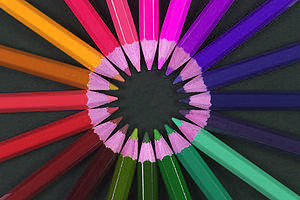
\includegraphics[height=0.65\textheight]{./output/ps1-2-a-1.png}
			\caption{ps1-2-a-1.png} 
		\end{figure}	
		
	\end{frame}

	\begin{frame}
		\frametitle{2b. Monochrome Green}
		
		\begin{figure}[!htb]
			\centering
			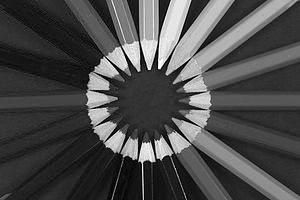
\includegraphics[height=0.65\textheight]{./output/ps1-2-b-1.png}
			\caption{Img1\_green - ps1-2-b-1.png} 
		\end{figure}	
		
	\end{frame}

	\begin{frame}
		\frametitle{2c. Monochrome Red}
		
		\begin{figure}[!htb]
			\centering
			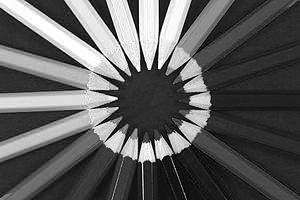
\includegraphics[height=0.65\textheight]{./output/ps1-2-c-1.png}
			\caption{Img1\_red - ps1-2-c-1.png} 
		\end{figure}	
		
	\end{frame}

	\begin{frame}
		\frametitle{3a. Replacement of Pixels}
		
		\begin{figure}[!htb]
			\centering
			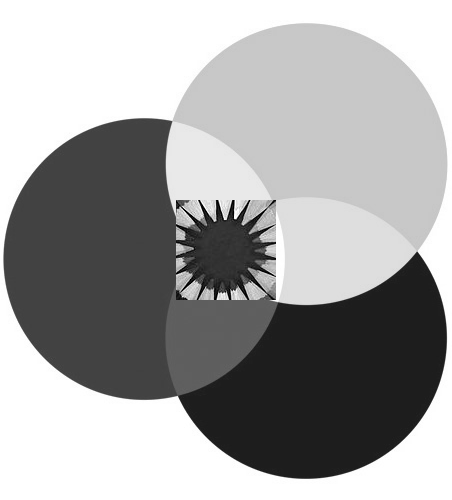
\includegraphics[height=0.65\textheight]{./output/ps1-3-a-1.png}
			\caption{ps1-3-a-1.png} 
		\end{figure}	
		
	\end{frame}

	\begin{frame}[t]
		\frametitle{4a. Image Stats}
		
		\begin{LARGE}
			\begin{itemize}
				\item Min = 0.0
				\item Max = 255.0
				\item Mean = 75.101033333333334
				\item Standard Deviation = 59.58611269078466
			\end{itemize}
		\end{LARGE}
		
	\end{frame}

	\begin{frame}
		\frametitle{4b. Arithmetic Operation}
		
		\begin{figure}[!htb]
			\centering
			
\includegraphics[height=0.65\textheight]{./output/ps1-4-b-1.png}
			\caption{ps1-4-b-1.png} 
		\end{figure}	
		
	\end{frame}

	\begin{frame}
		\frametitle{4c. Shifted Image}
		
		\begin{figure}[!htb]
			\centering
			
\includegraphics[height=0.65\textheight]{./output/ps1-4-c-1.png}
			\caption{ps1-4-c-1.png} 
		\end{figure}	
		
	\end{frame}	

	\begin{frame}
		\frametitle{4d. Difference Image}
		
		\begin{figure}[!htb]
			\centering
			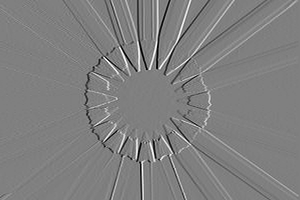
\includegraphics[height=0.65\textheight]{./output/ps1-4-d-1.png}
			\caption{ps1-4-d-1.png} 
		\end{figure}	
		
	\end{frame}

	\begin{frame}
		\frametitle{5a. Noisy Green Channel}
		
		\begin{figure}[!htb]
			\centering
			
\includegraphics[height=0.65\textheight]{./output/ps1-5-a-1.png}
			\caption{ps1-5-a-1.png} 
		\end{figure}	
		
	\end{frame}

	\begin{frame}
		\frametitle{5b. Noisy Blue Channel}
		
		\begin{figure}[!htb]
			\centering
			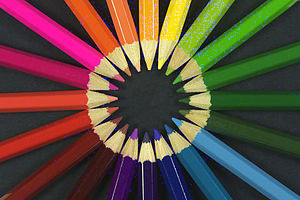
\includegraphics[height=0.65\textheight]{./output/ps1-5-b-1.png}
			\caption{ps1-5-b-1.png} 
		\end{figure}	
		
	\end{frame}

	\begin{frame}[t]
		\frametitle{6. Discussion}
		
		\begin{normalsize}
			\begin{itemize}
				\setlength\itemsep{1em}
				
				\item[a.] \textbf{Between all color channels, which channel, in your opinion, most resembles a gray-scale conversion of the original.  Why do you think this?  Does it matter for each respective image? (For this problem, you will have to read a bit on how the eye works/cameras to discover which channel is more prevalent and widely used)}
				
				\item[] It could be that humans are mostly sensitive to wavelengths spanning the green color spectrum which might be seen as the brightest of other colors [1]   

				\item[][1] http://light-measurement.com/spectral-sensitivity-of-eye/ % TODO
			\end{itemize}
		\end{normalsize}
		
	\end{frame}

	\begin{frame}[t]
		\frametitle{6. Discussion}
		
		\begin{normalsize}
			\begin{itemize}
				\setlength\itemsep{1em}
				
				\item[b.] \textbf{What does it mean when an image has negative pixel values stored?  Why is it important to maintain negative pixel values?}
				
				\item[] It means that the pixel with the negative value is relatively darker than those pixels with a more positive value. If no negative values were allowed and we were restricted with only uint8 numbers, we would lose information if we were to measure the difference between two pixels resulting in a negative value. This is because the negative values are converted to zeros and information is lost (e.g. -20 will be the same as -1 which is not accurate)
				
			\end{itemize}
		\end{normalsize}
		
	\end{frame}

	\begin{frame}[t]
		\frametitle{6. Discussion}
		
		\begin{normalsize}
			\begin{itemize}
				\setlength\itemsep{1em}
				
				\item[c.] \textbf{In question 5, noise was added to the green channel and also to the blue channel.  Which looks better to you? Why?  What sigma was used to detect any discernible difference?}

				\item[] The blue channel is better than the green channel and it is due to the same reason mentioned in 6a which is that human vision is more sensitive to wavelengths of the green spectrum. Sigma of 8 started to show blue noise on the noisy blue channel but it is much more tolerable than the green channel.
				
			\end{itemize}
		\end{normalsize}
		
	\end{frame}
	
\end{document}